\section{Pausing environment}
\label{sec:pause}

We first formally define the simplified syntax of \Hazel shown in Figure \ref{fig:syntax} \cite{HazelLive}. The symbol $\ehole$ represents the empty hole used to indicate the place where missing piece is. And for the expression that doesn't have clear meaning, we use $\llparenthesiscolor e \rrparenthesiscolor$ to indicate that it doesn't have semantic meanings. We only consider binary sums so for $\hinj{i}{e}$,  $i$ is in set $\{L, R\}$.

\begin{figure}[htbp]
    \vspace{-3px} 
  $\arraycolsep=4pt\begin{array}{lll}
  HTyp~~ \tau & ::= &
    \tnum  ~\vert~
    \tarr{\tau}{\tau} ~\vert~
    (\tau + \tau) ~\vert~
    \ehole
    \\
  HExp~~ e & ::= &
    x ~\vert~
    \lamfunc{x}{e} ~\vert~
    \lamfunc{x:\tau}{e} ~\vert~
    e(e) ~\vert~
    \underlinenum{n} ~\vert~
    (e+e) ~\vert~
    e: \tau ~\vert~
    \hinj{i}{e} ~\vert~
    \hcase{e}{x}{e}{y}{e}~\vert~
    \ehole  ~\vert~
    \notehole{e} 
  \end{array}$
  \hrule
  \caption{Syntax of H-types, H-expressions}
    \label{fig:syntax}
    \vspace{-5px}
\end{figure}

\begin{figure}[htbp]
    \vspace{-3px} 
    \fbox{ $\isPaused{e} $}~~\text{$e$ is paused}\hfill
    \begin{subequations}\label{eqns:paused}
    \begin{mathpar}
        \hfill
        \inferrule[PCase]{ \isIndet{e_0}
            }{
              \isPaused{\hap{\lamfunc{z}{\hcase{z}{x}{e_1}{y}{e_2}}}{e_0}}
            }
        \hfill
        \inferrule[PAp1]{ \isPaused{e_1}
            }{
              \isPaused{\hap{e_1}{e_2}}
            }
        \hfill
        \inferrule[PAp2]{ \isPaused{e_2}
            }{
              \isPaused{\hap{e_1}{e_2}}
            }
        \hfill
        \cdots
        \hfill
        \hfill
    \end{mathpar}
    
    \end{subequations}
    \caption{Paused forms}
    \label{fig:paused_forms}
    \vspace{-5px}
\end{figure}

\HazelnutLive, an editor for \Hazel, defines judgement like $\isFinal{e}$, $\isBoxed{e}$ for expression $e$ \cite{HazelLive}. Furthermore, since \Hazel contains incomplete programs, there exist some indeterminate programs, which induces a judgement denoted as $\isIndet{e}$.

Pausing judgement is denoted as $\isPaused{e}$. This paused judgement is designed to simplify the output of the program since \Hazel has some complicated programs that can not be evaluated further. Therefore, the paused expression is steppable but this needs user's confirmation. For example, we want to avoid the long cases as output. Therefore, when $\ehole$ appears at case expression so that the match algorithm gives indeterminate result, it will be a paused expression stopping the stepper immediately. The judgement is shown in Figure \ref{fig:paused_forms}. $\mathtt{PCase}$ is the case that the output will be long and useless. Other rules make paused judgement propagate up. Besides, this judgement can also be extended in the future. For example, function with multiple arguments should pause before it goes into beta rule. Otherwise, it is wired to see a partial function when there is only one argument given.


%Figure \ref{fig:pause} gives a expression as example. It defines a function func. But we don't provide any argument for it. The evaluator expand the case expression directly. However, the result in bottom shows an example that when augment is only a hole, the stepper will not evaluate but stop with yellow box indicating it is steppable but paused.

% \begin{figure}[htbp]
%     \centering
%     \begin{subfigure}[b]{0.4\textwidth}
%         \centering
%         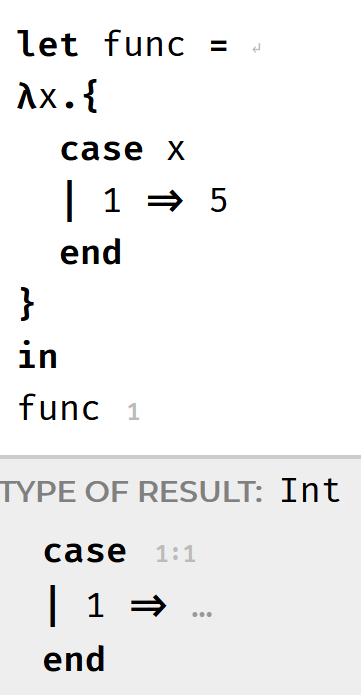
\includegraphics[width=0.4\textwidth]{img/case1.png}
%         \caption{}
%         \label{fig:pause1}
%     \end{subfigure}
%     \begin{subfigure}[b]{0.4\textwidth}
%         \centering
%         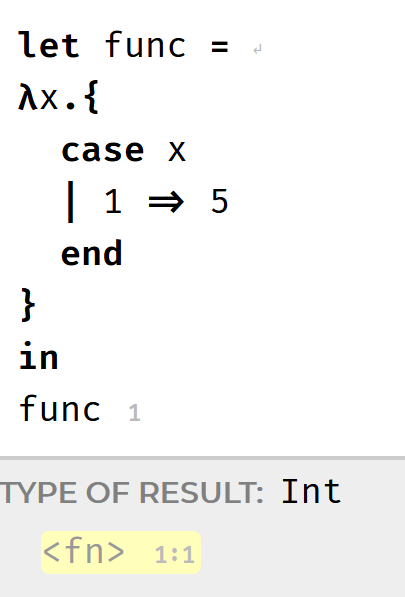
\includegraphics[width=0.5\textwidth]{img/case2.png}
%         \caption{}
%         \label{fig:pause2}
%     \end{subfigure}
%     \caption{Example of stepper with paused environment}
% \end{figure}